\documentclass[12pt]{beamer}
\usepackage{cmap}
\usepackage[T2A]{fontenc}
\usepackage[utf8]{inputenc}
\usepackage{ifluatex}
\usefonttheme[onlymath]{serif}
\usepackage{svg}
\usepackage{enumerate}
\usepackage{hyperref}
\usepackage{mathtools}

\definecolor{beamer@darkgreen}{rgb}{0,0.6,0}
\setbeamercolor{normal text}{fg=black,bg=white}
\setbeamercolor{title}{fg=black,bg=beamer@darkgreen}
\setbeamercolor{frametitle}{fg=black,bg=beamer@darkgreen}
\setbeamercolor{background canvas}{parent=normal text}

\usepackage[english,russian]{babel}
\usepackage{graphicx}
\usepackage{listings}

\author{Катя Тузова}
\title{Машинное обучение}
\subtitle{Лекция 3. Методы кластеризации}
\date{}

\begin{document}
\frame{\titlepage}

\begin{frame}\frametitle{Разбор летучки}
	Что такое прецедент?
\end{frame}

\begin{frame}\frametitle{Разбор летучки}
	Задача обучения с учителем.\\
	\vspace{5mm}
	Множество объектов $X$ \\
	Множество допустимых ответов $Y$\\
	Прецедент - пара объект-ответ ${(x_i,y_i)}$  \\
	$x_i \in X$ 	$y_i \in Y$
\end{frame}

\begin{frame}\frametitle{Разбор летучки}
	К какому типу задач относятся:
	\begin{itemize}
		\item[--] Прогнозирования потребительского спроса. У компании есть 1000 продуктов, которые она производит. Требуется предсказать сколько будет продано в следующие полгода.
		% регрессия
		\item[--] Вы владелец фейсбука и пишете алгоритм, который определяет был ли взломан пользователь. 
		% классификация
		\item[--] В задачах медицинской диагностики в роли объектов выступают пациенты. Найти вид заболевания.
		%классификация
		\item[--] Задача кредитного скоринга (Оценка кредитоспособности клиента, на основании которой принимается решение о выдаче кредита)
		% классификация
	\end{itemize}
\end{frame}

\begin{frame}\frametitle{Разбор летучки}
	К какому типу задач относятся:
	\begin{itemize}
		\item[--] Прогнозирования потребительского спроса. 
\textcolor{red}{(регрессия)}
		\item[--] Взломан ли пользователь. \textcolor{red}{(бинарная классификация)}
		\item[--] Найти вид заболевания. \textcolor{red}{(классификация)}
		\item[--] Задача кредитного скоринга.  \textcolor{red}{(классификация)}
	\end{itemize}
\end{frame}

\begin{frame}\frametitle{Разбор летучки}
Какие из следующих задач являются задачей обучения без учителя?
\begin{itemize}
	\item[--] Спам фильтр
	\item[--] Рубрикация текстов (Группировка статей по темам)
	\item[--] Оценить есть ли у нового пациента диабет
	\item[--] Прогнозирование времени следующего землетрясения на определенной территории.
	\item[--] Разделение людей по психотипу. 
\end{itemize}
\end{frame}

\begin{frame}\frametitle{Разбор летучки}
Какие из следующих задач являются задачей обучения без учителя?
\begin{itemize}
	\item[--] Спам фильтр
	\item[+] Рубрикация текстов (Группировка статей по темам)
	\item[--] Оценить есть ли у нового пациента диабет
	\item[--] Прогнозирование времени следующего землетрясения на определенной территории.
	\item[+] Разделение людей по психотипу. 
\end{itemize}
\end{frame}

\begin{frame}\frametitle{Разбор летучки}
\begin{itemize}
\item[--] Пол
\item[--] Средний школьный балл
\item[--] Номер школы
\item[--] Город школы
\item[--] Доля пропущенных лекций
\item[--] Оценка по мнению родителей
\item[--] Пиво/неделя
\item[--] Друзей в ВКонтакте
\item[--] Расстояние от дома до универа
\item[--] Ряд в аудитории
\item[--] Наличие планшета
\item[--] Периметр головы
\end{itemize}
\end{frame}

\begin{frame}\frametitle{Разбор летучки}
\begin{itemize}
\item[--] Пол \textcolor{red}{(бинарный)}
\item[--] Средний школьный балл \textcolor{red}{(количественный)}
\item[--] Номер школы \textcolor{red}{(номинальный)}
\item[--] Город школы  \textcolor{red}{(номинальный)}
\item[--] Доля пропущенных лекций   \textcolor{red}{(количественный)}
\item[--] Оценка по мнению родителей   \textcolor{red}{(порядковый)}
\item[--] Пиво/неделя    \textcolor{red}{(количественный)}
\item[--] Друзей в ВКонтакте   \textcolor{red}{(количественный)}
\item[--] Расстояние от дома до универа  \textcolor{red}{(количественный)}
\item[--] Ряд в аудитории  \textcolor{red}{(порядковый)}
\item[--] Наличие планшета  \textcolor{red}{(бинарный)}
\item[--] Периметр головы   \textcolor{red}{(количественный)}
\end{itemize}
\end{frame}

\begin{frame}\frametitle{Разбор летучки}
Приведите пример переобучения и недообучения.
\end{frame}

\begin{frame}\frametitle{Разбор летучки}
Приведите пример переобучения и недообучения.
\begin{figure}[htbp]
  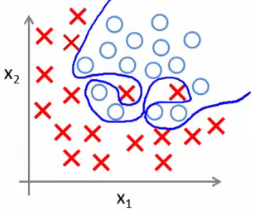
\includegraphics[height=100pt, keepaspectratio = true]{images/overfitting}  
  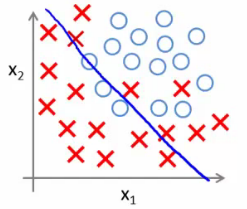
\includegraphics[height=100pt, keepaspectratio = true]{images/underfitting}  
\end{figure}
\end{frame}

\begin{frame}\frametitle{Разбор летучки 2}
Что такое cross-fold validation? 
\end{frame}

\begin{frame}\frametitle{Разбор летучки 2}
Что такое cross-fold validation? \\
\vspace{5mm}
Способ разбиения обучающей выборки на два множества $L$ и $T$.
\end{frame}

\begin{frame}\frametitle{Разбор летучки 2}
\textbf{Гипотеза компактности:}\\
Схожие объекты, как правило, лежат в одном классе.\\
\end{frame}

\begin{frame}\frametitle{Разбор летучки 2}
${a(u, X^l) = \arg\max_{y \in Y} \underbrace{\sum\limits_{i=1}^l [y_u^i = y]w(i, u)}_{\Gamma_y(u)} }$\\
Смысл параметров $w$, $i$, $u$, $\Gamma_y(u)$
\end{frame}

\begin{frame}\frametitle{Разбор летучки 2}
${a(u, X^l) = \arg\max_{y \in Y} \underbrace{\sum\limits_{i=1}^l [y_u^i = y]w(i, u)}_{\Gamma_y(u)} }$\\
$w(i, u)$ - вес $i$-го соседа $u$ \\
$i$ - порядковый номер соседа $u$ в упорядоченном множестве\\
$u$ -- объект, для которого проводится классификация\\
$\Gamma_y(u)$ -- оценка близости объекта $u$ к классу ${y}$
\end{frame}

\begin{frame}\frametitle{Разбор летучки 2}
Мотивация для использования Парзеновского окна. В чем минусы зависимости веса объекта только от его порядкового номера?
\end{frame}

\begin{frame}\frametitle{Разбор летучки 2}
Мотивация для использования Парзеновского окна. В чем минусы зависимости веса объекта только от его порядкового номера?\\
\vspace{5mm}
Объекты, находящиеся на одинаковом расстоянии будут взяты с разными весами. 
Далекие объекты могут быть взяты со слишком большим весом.
\end{frame}

\begin{frame}\frametitle{Разбор летучки 2}
Какими свойствами должна обладать функция $K$, чтобы использовать ее в качестве ядра?
\end{frame}

\begin{frame}\frametitle{Разбор летучки 2}
Какими свойствами должна обладать функция $K$, чтобы использовать ее в качестве ядра?\\
\vspace{5mm}
Невозрастающая функция, положительная на отрезке [0, 1]
\end{frame}

\begin{frame}\frametitle{Разбор летучки 2}
      Что по оси ординат? \\
   \begin{minipage}[t]{0.35\linewidth}

	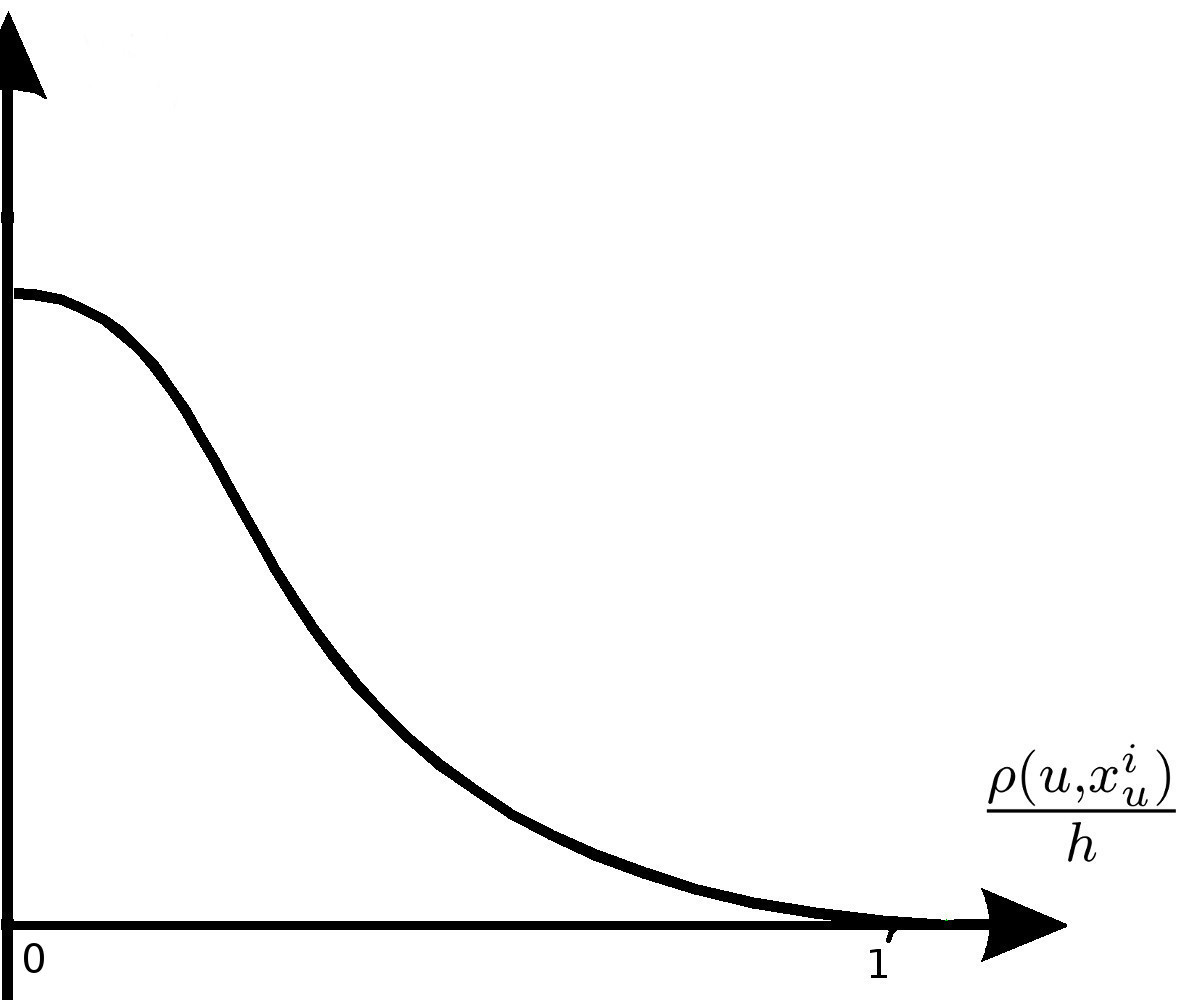
\includegraphics[height=150px]{images/parzen}
   \end{minipage}
\end{frame}

\begin{frame}\frametitle{Разбор летучки 2}
      Что по оси ординат? \\
   \begin{minipage}[t]{0.35\linewidth}

	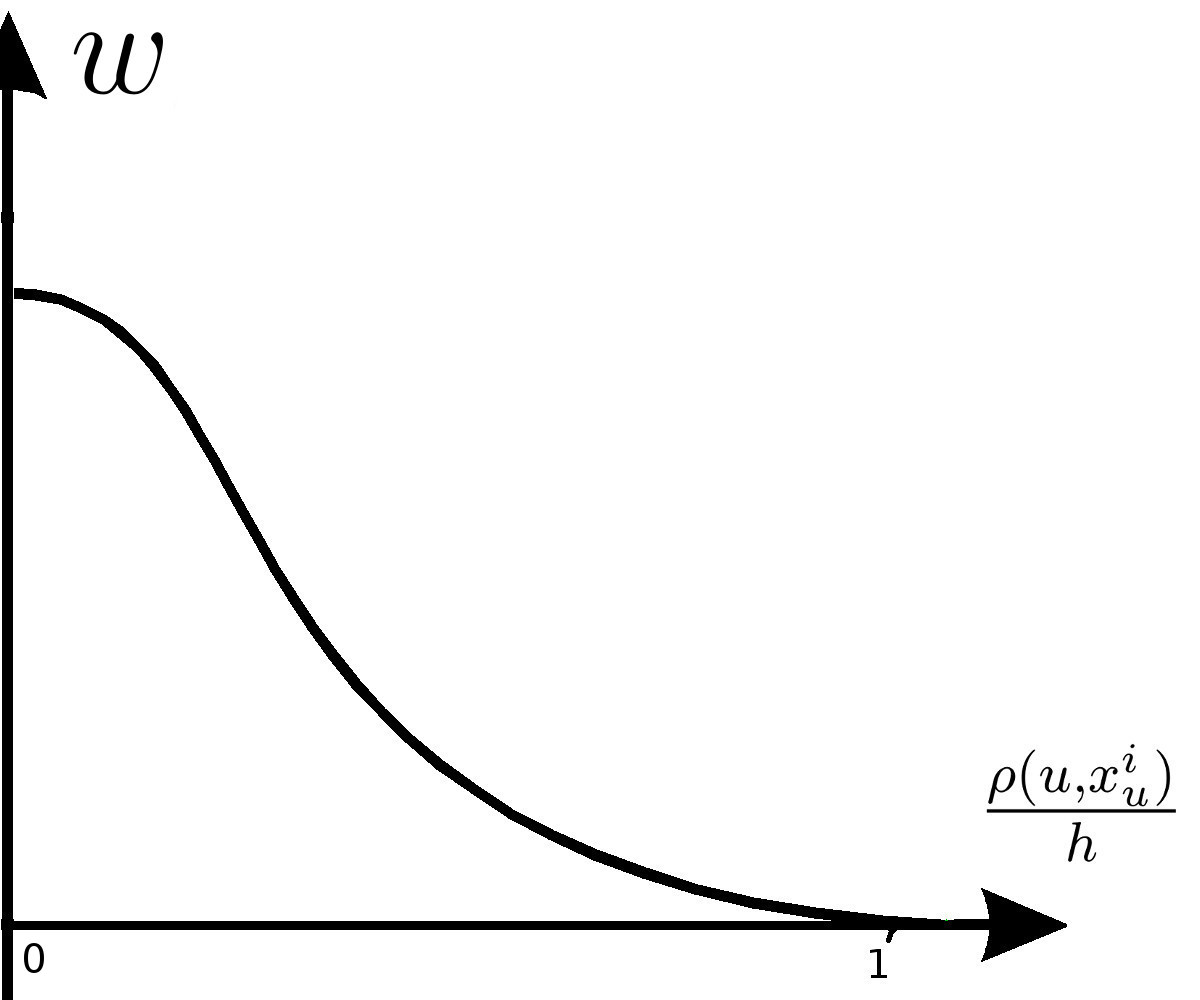
\includegraphics[height=150px]{images/parzen1}
   \end{minipage}
\end{frame}

\begin{frame}\frametitle{Разбор летучки 2}
Как подбирать функцию расстояния?
\end{frame}
 
\begin{frame}\frametitle{Разбор летучки 2}
Как подбирать функцию расстояния?\\
\vspace{5mm}
Максимизировать сумму расстояний между объектами разных классов
при этом сохраняя сумму расстояний между объектами одного класса небольшой.\\
\vspace{8mm}
${\max \sum_{x_i, x_j \in D} \rho(x_i, x_j) }$\\
\vspace{8mm}
%${\sum_{x_i, x_j \in S} d_M^2(x_i, x_j) \leq 1 }$
${\sum_{x_i, x_j \in S} \rho^2(x_i, x_j) \leq 1 }$
\end{frame}
 
\begin{frame}\frametitle{Разбор летучки 2}
Что такое проклятие размерности?
\end{frame}

\begin{frame}\frametitle{Разбор летучки 2}
Что такое проклятие размерности?\\
\vspace{5mm}

Если используемая метрика
${\rho(u, x_u^i)}$
основана на суммировании различий по всем признакам, а число признаков очень велико,
то все точки выборки могут оказаться практически одинаково
далеки друг от друга.\\
\end{frame}

\begin{frame}\frametitle{Разбор летучки 2}
Жадное добавление признаков -- как определить, что признаков уже достаточно?
\end{frame}

\begin{frame}\frametitle{Разбор летучки 2}
Жадное добавление признаков -- как определить, что признаков уже достаточно?\\
\vspace{5mm}
Все время минимизируем функционал скользящего контроля (leave-one-out):\\
${LOO(k, X^l) = \sum\limits_{i=1}^l [a(x_i; X^l \backslash \left\{x_i\right\}, k) \neq y] \rightarrow \min_k}$\\
Добавляем признаки, пока LOO не увеличивается
\end{frame}

\begin{frame}\frametitle{Разбор летучки 2}
Чем эталонный объект отличается от надежно классифицируемого?\\
\end{frame}

\begin{frame}\frametitle{Разбор летучки 2}
Чем эталонный объект отличается от надежно классифицируемого?\\
\vspace{8mm}
Эталонные объекты имеют большой положительный отступ, плотно окружены
объектами своего класса и являются наиболее типичными его представителями.\\
\vspace{5mm}
Надежно классифицируемые(неинформативные) объекты -- изъятие
этих объектов из выборки не влияет на качество классификации. Фактически, они не добавляют к эталонам никакой новой информации. 

\end{frame}

\begin{frame}\frametitle{Быстрый поиск ближайшего соседа}
\end{frame}

\begin{frame}\frametitle{k-d дерево}
Идея: разложим множество по поторому будем искать
в бинарное дерево с простыми условиями и
конкретными точками в узлах.
\vspace{5mm}
\begin{enumerate}
\item По циклу, или рандомно выбираем ось.
\item Ищем точку, разбивающую множество на как
можно более равные части.
\item Повторяем 1-2 для каждого из получившихся подмножеств 
\end{enumerate}
Сложность построения: $O(n\log n)$\\
Сложность поиска: в лучшем
случае $O(\log n)$, в худшем -- $O(n)$
\end{frame}
\begin{frame}\frametitle{2-d дерево}

\begin{figure}[htbp]
\centering
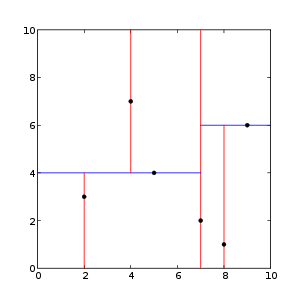
\includegraphics[height=190pt]{images/Kdtree_2d}  
\end{figure}
\end{frame}

\begin{frame}\frametitle{k-d дерево. Особенности}
\begin{itemize}
\item[+] Один из наиболее простых методов
\item[--] Работает только при малом количестве параметров
\item[--] Затратный алгоритм перестроения

\end{itemize}
\end{frame}

\begin{frame}\frametitle{Locality Sensitive Hash}
R-соседи -- соседи в радиусе R от объекта.\\
\vspace{5mm}
Хэш-функция $h(R, cR, p1, p2)$:\\
$\Vert u - v \Vert  \leq R => p(h(u) = h(v)) \geq p_1$ \\
$\Vert u - v \Vert  \geq cR => p(h(u) = h(v)) \leq p_2$ 
\end{frame}

\begin{frame}\frametitle{Постановка задачи кластеризации}
Кластеризация -- задача разделения объектов одной природы на несколько групп так, чтобы объекты в одной группе обладали одним и тем же свойством.\\
\vspace{5mm}
Кластеризация -- это обучение без учителя.
\end{frame}

\begin{frame}\frametitle{Постановка задачи кластеризации}
$X$ -- пространство объектов\\
$X^l$ = $\left\{ x\right\}_{i=1}^l$ -- обучающая выборка\\
$\rho: X \times X \rightarrow [0, \infty)$ -- функция расстояния между объектами\\
\vspace{5mm}
Найти:\\
$Y$ -- множество кластеров \\
$a: X \rightarrow Y$ -- алгоритм кластеризации
\vspace{5mm}

\end{frame}

\begin{frame}\frametitle{Степени свободы в постановке задачи}
\end{frame}

\begin{frame}\frametitle{Степени свободы в постановке задачи}
	\begin{itemize}
		\item[--] Критерий качества кластеризации
		\item[--] Число кластеров неизвестно заранее
		\item[--] Результат кластеризации существенно зависит от метрики
	\end{itemize}
\end{frame}

\begin{frame}\frametitle{Цели кластеризации}
\end{frame}

\begin{frame}\frametitle{Цели кластеризации}
	\begin{itemize}
		\item[--] Сократить объём хранимых данных
		\item[--] Выделить нетипичные объекты
		\item[--] Упростить дальнейшую обработку данных
		\item[--] Построить иерархию множества объектов				
	\end{itemize}
\end{frame}

\begin{frame}\frametitle{Какие бывают кластеры?}
\end{frame}

\begin{frame}\frametitle{Типы кластерных структур. Сгущения}
\begin{figure}[htbp]
  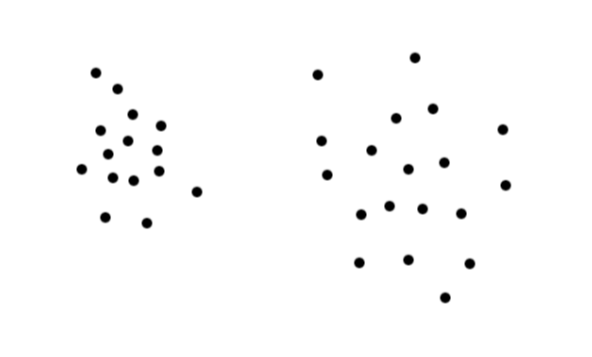
\includegraphics[height=130pt, keepaspectratio = true]{images/cluster1}  
\end{figure}
\end{frame}

\begin{frame}\frametitle{Типы кластерных структур. Ленты}
\begin{figure}[htbp]
  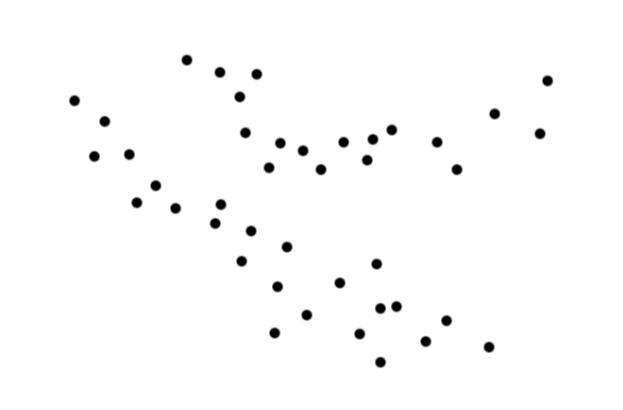
\includegraphics[height=130pt, keepaspectratio = true]{images/cluster2}  
\end{figure}
\end{frame}

\begin{frame}\frametitle{Типы кластерных структур. С центром}
\begin{figure}[htbp]
  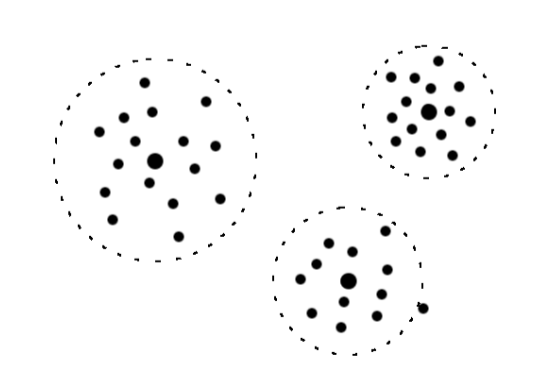
\includegraphics[height=130pt, keepaspectratio = true]{images/cluster3}  
\end{figure}
\end{frame}

\begin{frame}\frametitle{Типы кластерных структур. С перемычками}
\begin{figure}[htbp]
  
\includegraphics[height=130pt, keepaspectratio = true]{images/cluster4}  
\end{figure}
\end{frame}

\begin{frame}\frametitle{Типы кластерных структур. На фоне}
\begin{figure}[htbp]
  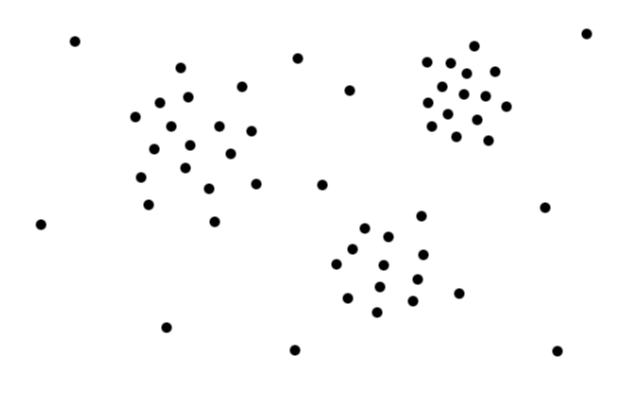
\includegraphics[height=130pt, keepaspectratio = true]{images/cluster5}  
\end{figure}
\end{frame}

\begin{frame}\frametitle{Типы кластерных структур. Перекрывающиеся}
\begin{figure}[htbp]
  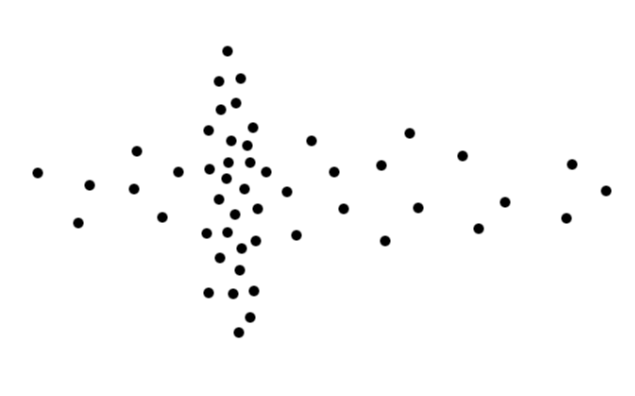
\includegraphics[height=130pt, keepaspectratio = true]{images/cluster6}  
\end{figure}
\end{frame}

\begin{frame}\frametitle{Чувствительность к выбору метрики}
\begin{figure}[htbp]
  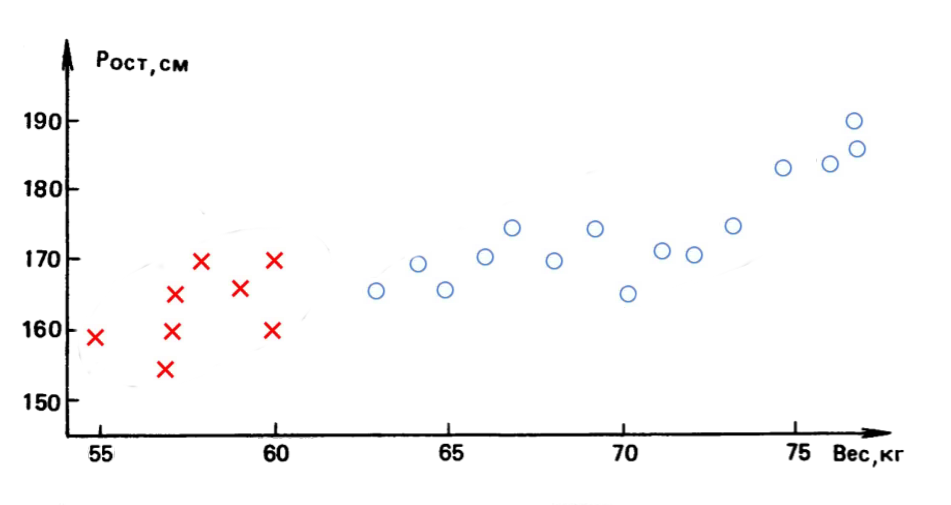
\includegraphics[height=160pt, keepaspectratio = true]{images/students}  
\end{figure}
\end{frame}

\begin{frame}\frametitle{Чувствительность к выбору метрики}
\begin{figure}[htbp]
  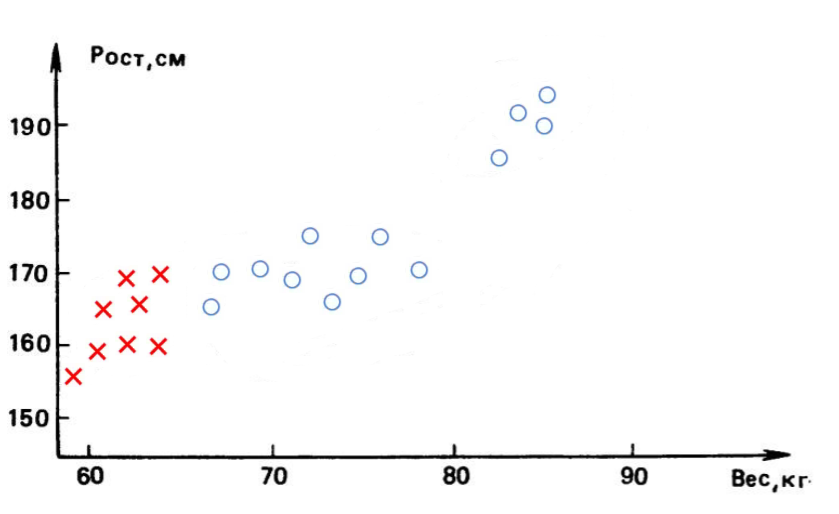
\includegraphics[height=160pt, keepaspectratio = true]{images/students1}  
\end{figure}
\end{frame}

\begin{frame}\frametitle{Оценка качества кластеризации}
Есть несколько разбиений на кластеры. Как их сравнить?
\end{frame}

\begin{frame}\frametitle{Оценка качества кластеризации}
\begin{itemize}
\item[--] Минимизировать среднее внутрикластерное расстояние\\
\vspace{5mm}
${\frac{\sum_{a(x_i) = a(x_j)} \rho(x_i, x_j)}{\sum_{a(x_i) = a(x_j)} 1} \rightarrow \min}$
\item[--] Максимизировать среднее межкластерное расстояние\\
\vspace{5mm}
${\frac{\sum_{a(x_i) \neq a(x_j)} \rho(x_i, x_j)}{\sum_{a(x_i) \neq a(x_j)} 1} \rightarrow \max}$
\end{itemize}
\end{frame}

\begin{frame}\frametitle{Методы кластеризации}
\begin{itemize}
\item[--] Иерархические
\item[--] Графовые 
\item[--] Статистические 
\end{itemize}
\end{frame}

\begin{frame}\frametitle{Иерархическая кластеризация}

\end{frame}

\begin{frame}\frametitle{Графовые алгоритмы}
Очевидные:\\
\begin{itemize}
\item[--] Выделение связных компонент
\item[--] Минимальное покрывающее дерево
\end{itemize}
\end{frame}

\begin{frame}\frametitle{Расстояние между кластерами. Формула Ланса-Уильямса}
\end{frame}

\begin{frame}\frametitle{Увеличение эффективности Ланса-Уильямса}
\end{frame}

\begin{frame}\frametitle{Визуализация кластеров. Дендрограмма}
\end{frame}

\begin{frame}\frametitle{Визуализация кластеров. Диаграмма вложения}
\end{frame}

\begin{frame}\frametitle{Свойство монотонности}
\end{frame}

\begin{frame}\frametitle{Визуализация кластеров. Диаграмма вложения}
\end{frame}

\begin{frame}\frametitle{Метод $k$-средних}
\end{frame}

\begin{frame}\frametitle{Модификации метода $k$-средних}
\end{frame}

\begin{frame}\frametitle{Плюсы и минусы метода $k$-средних}
\end{frame}

%\begin{frame}\frametitle{Карты Кохонена}
% нельзя без нейросетей
%\end{frame}

\end{document}
